\documentclass[tikz,border=5pt]{standalone}
\usepackage[T1]{fontenc}
\usepackage{lmodern}
\usepackage{amsmath}
\usetikzlibrary{arrows.meta,positioning,calc}

\definecolor{orblue}{RGB}{76,120,168}
\definecolor{ororange}{RGB}{209,143,0}
\definecolor{orgray}{RGB}{122,122,122}

\begin{document}
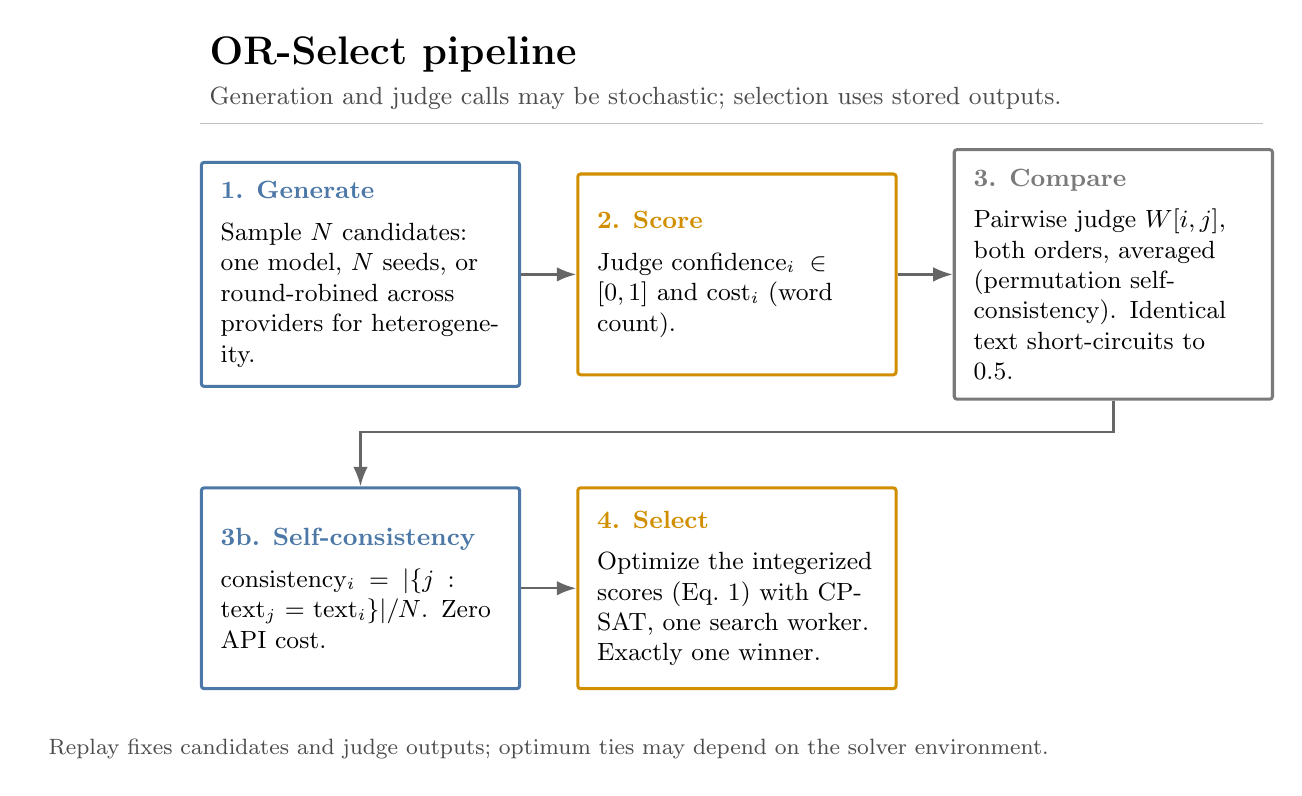
\begin{tikzpicture}[
  >=Latex,
  flow/.style={-Latex,draw=black!60,line width=0.9pt},
  box/.style={fill=white,line width=1.1pt,rounded corners=1pt,
    text width=3.55cm,minimum height=2.55cm,align=left,inner sep=7pt,
    font=\small},
  note/.style={font=\footnotesize,text=black!70,align=center}
]
\node[anchor=west,font=\Large\bfseries] at (0,0) {OR-Select pipeline};
\node[anchor=west,font=\small,text=black!70] at (0,-0.55)
  {Generation and judge calls may be stochastic; selection uses stored outputs.};
\draw[black!25] (0,-0.88) -- (13.5,-0.88);

\node[box,draw=orblue,anchor=north west] (gen) at (0,-1.35) {
  \textcolor{orblue}{\textbf{1. Generate}}\\[4pt]
  Sample $N$ candidates: one model, $N$ seeds, or round-robined across providers for heterogeneity.};

\node[box,draw=ororange,right=0.7cm of gen] (score) {
  \textcolor{ororange}{\textbf{2. Score}}\\[4pt]
  Judge confidence$_i \in [0,1]$ and cost$_i$ (word count).};

\node[box,draw=orgray,right=0.7cm of score] (compare) {
  \textcolor{orgray}{\textbf{3. Compare}}\\[4pt]
  Pairwise judge $W[i,j]$, both orders, averaged (permutation self-consistency). Identical text short-circuits to $0.5$.};

\node[box,draw=orblue,below=1.25cm of gen] (consist) {
  \textcolor{orblue}{\textbf{3b. Self-consistency}}\\[4pt]
  consistency$_i = |\{j: \text{text}_j = \text{text}_i\}| / N$. Zero API cost.};

\node[box,draw=ororange,right=0.7cm of consist] (select) {
  \textcolor{ororange}{\textbf{4. Select}}\\[4pt]
  Optimize the integerized scores (Eq.~1) with CP-SAT, one search worker. Exactly one winner.};

\draw[flow] (gen.east) -- (score.west);
\draw[flow] (score.east) -- (compare.west);
\draw[flow] (compare.south) -- ++(0,-0.4) -| (consist.north);
\draw[flow] (consist.east) -- (select.west);

\node[note,anchor=north,text width=13cm] at ($(consist.south)!0.5!(select.south)+(0,-0.5)$)
  {Replay fixes candidates and judge outputs; optimum ties may depend on the solver environment.};
\end{tikzpicture}
\end{document}
